\providecommand*{\height}{h}
\providecommand*{\radius}{r}
\providecommand*{\volume}{v}

% ball
%
\providecommand*{\rball}{\radius\sbtxt{ball}}
\providecommand*{\vball}{\volume\sbtxt{ball}}

% cylinder
%
\providecommand*{\hcyl}{\height\sbtxt{cyl}}
\providecommand*{\rcyl}{\radius\sbtxt{cyl}}
\providecommand*{\vcyl}{\volume\sbtxt{cyl}}


\section{Archimedes's principle} % (fold)
\label{sec:archimedes_s_principle}
%
\subsection{Problem statement} % (fold)
\label{sub:problem_statement}
%
Consider a circular cylinder of height $\phi$ and radius $\rho$ and a ball of radius $\rho'$. Let the cylinder circumscribe the ball. Then, use triple integration to calculate the ball-cylinder volumetric ratio.

% subsection problem_statement (end)


\subsection{Problem statement analysis} % (fold)
\label{sub:problem_statement_analysis}
%
\theme{Analyze.} Look for some possible troubles with the problem statement.

\theme{Extreme cases.} The problem statement allows us to choose any ball (the cylinder follows by circumscription). Then, consider the empty ball. The empty cylinder thus circumscribes the empty ball. By definition, an empty figure has zero volume. Therefore, both empty figures have zero volume and their ratio just becomes
%
\begin{equation*}
  \dfrac\vball\vcyl = \dfrac 00 = \text{undefined!}
\end{equation*}
%
\theme{Need for reformulation.} Although a solution, this answer is not very useful for the general case (nonempty figures). So we have to reformulate the statement to limit math pathologies.

\theme{Suitable notation.} Additionally, the statement \emph{suggests} notation. But such a notation is not very intuitive. Then, since we are not forced to follow the \statusquo, we can choose more suitable notation at any time.

\theme{Suitable methodology.} Finally, the statement \emph{suggests} a solution path: calculus. But, as in the case of notation, we are not compelled to follow it. We aim then for a different statement that will free us to choose our own notation and methods. Hopefully, this will also help us to deepen in understanding, rather than to find \scare{correct} answers.

% subsection problem statement analysis (end)


\subsection{Problem statement reformulation} % (fold)
\label{sub:problem_statement_reformulation}
%
\theme{Reformulated problem.} \scare{Consider a nonempty cylinder and consider a nonempty ball. Let the cylinder circumscribe the ball. Then, find their volumetric ratio.} 

\theme{Critique.} This statement removes empty shapes and sets us free to select both notation and solving methodologies. Nevertheless, we can further improve it.

\theme{Be concise.} We only require a nonempty ball, since a nonempty cylinder will follow due to circumscription. We additionally join the clauses.

\theme{Reformulate statement.} We work therefore with a new statement:
%
\begin{quotation}
  Calculate the volumetric ratio of a circular cylinder circumscribing a nonempty ball.
\end{quotation}

% subsection problem_statement_reformulation (end)


\subsection{Terminology, figures, notation} % (fold)
\label{sub:terminology_and_notation}

\theme{Define terms before proceed.} To \lingo{circumscribe}: draw (a figure) around another, touching it at points but not cutting it. 

\theme{Depict.} When a cylinder circumscribes a ball, it meets the ball at six points as shown in \cref{fig:archimedes}.
%
\begin{figure}[b]
  \capstart
  \centering
  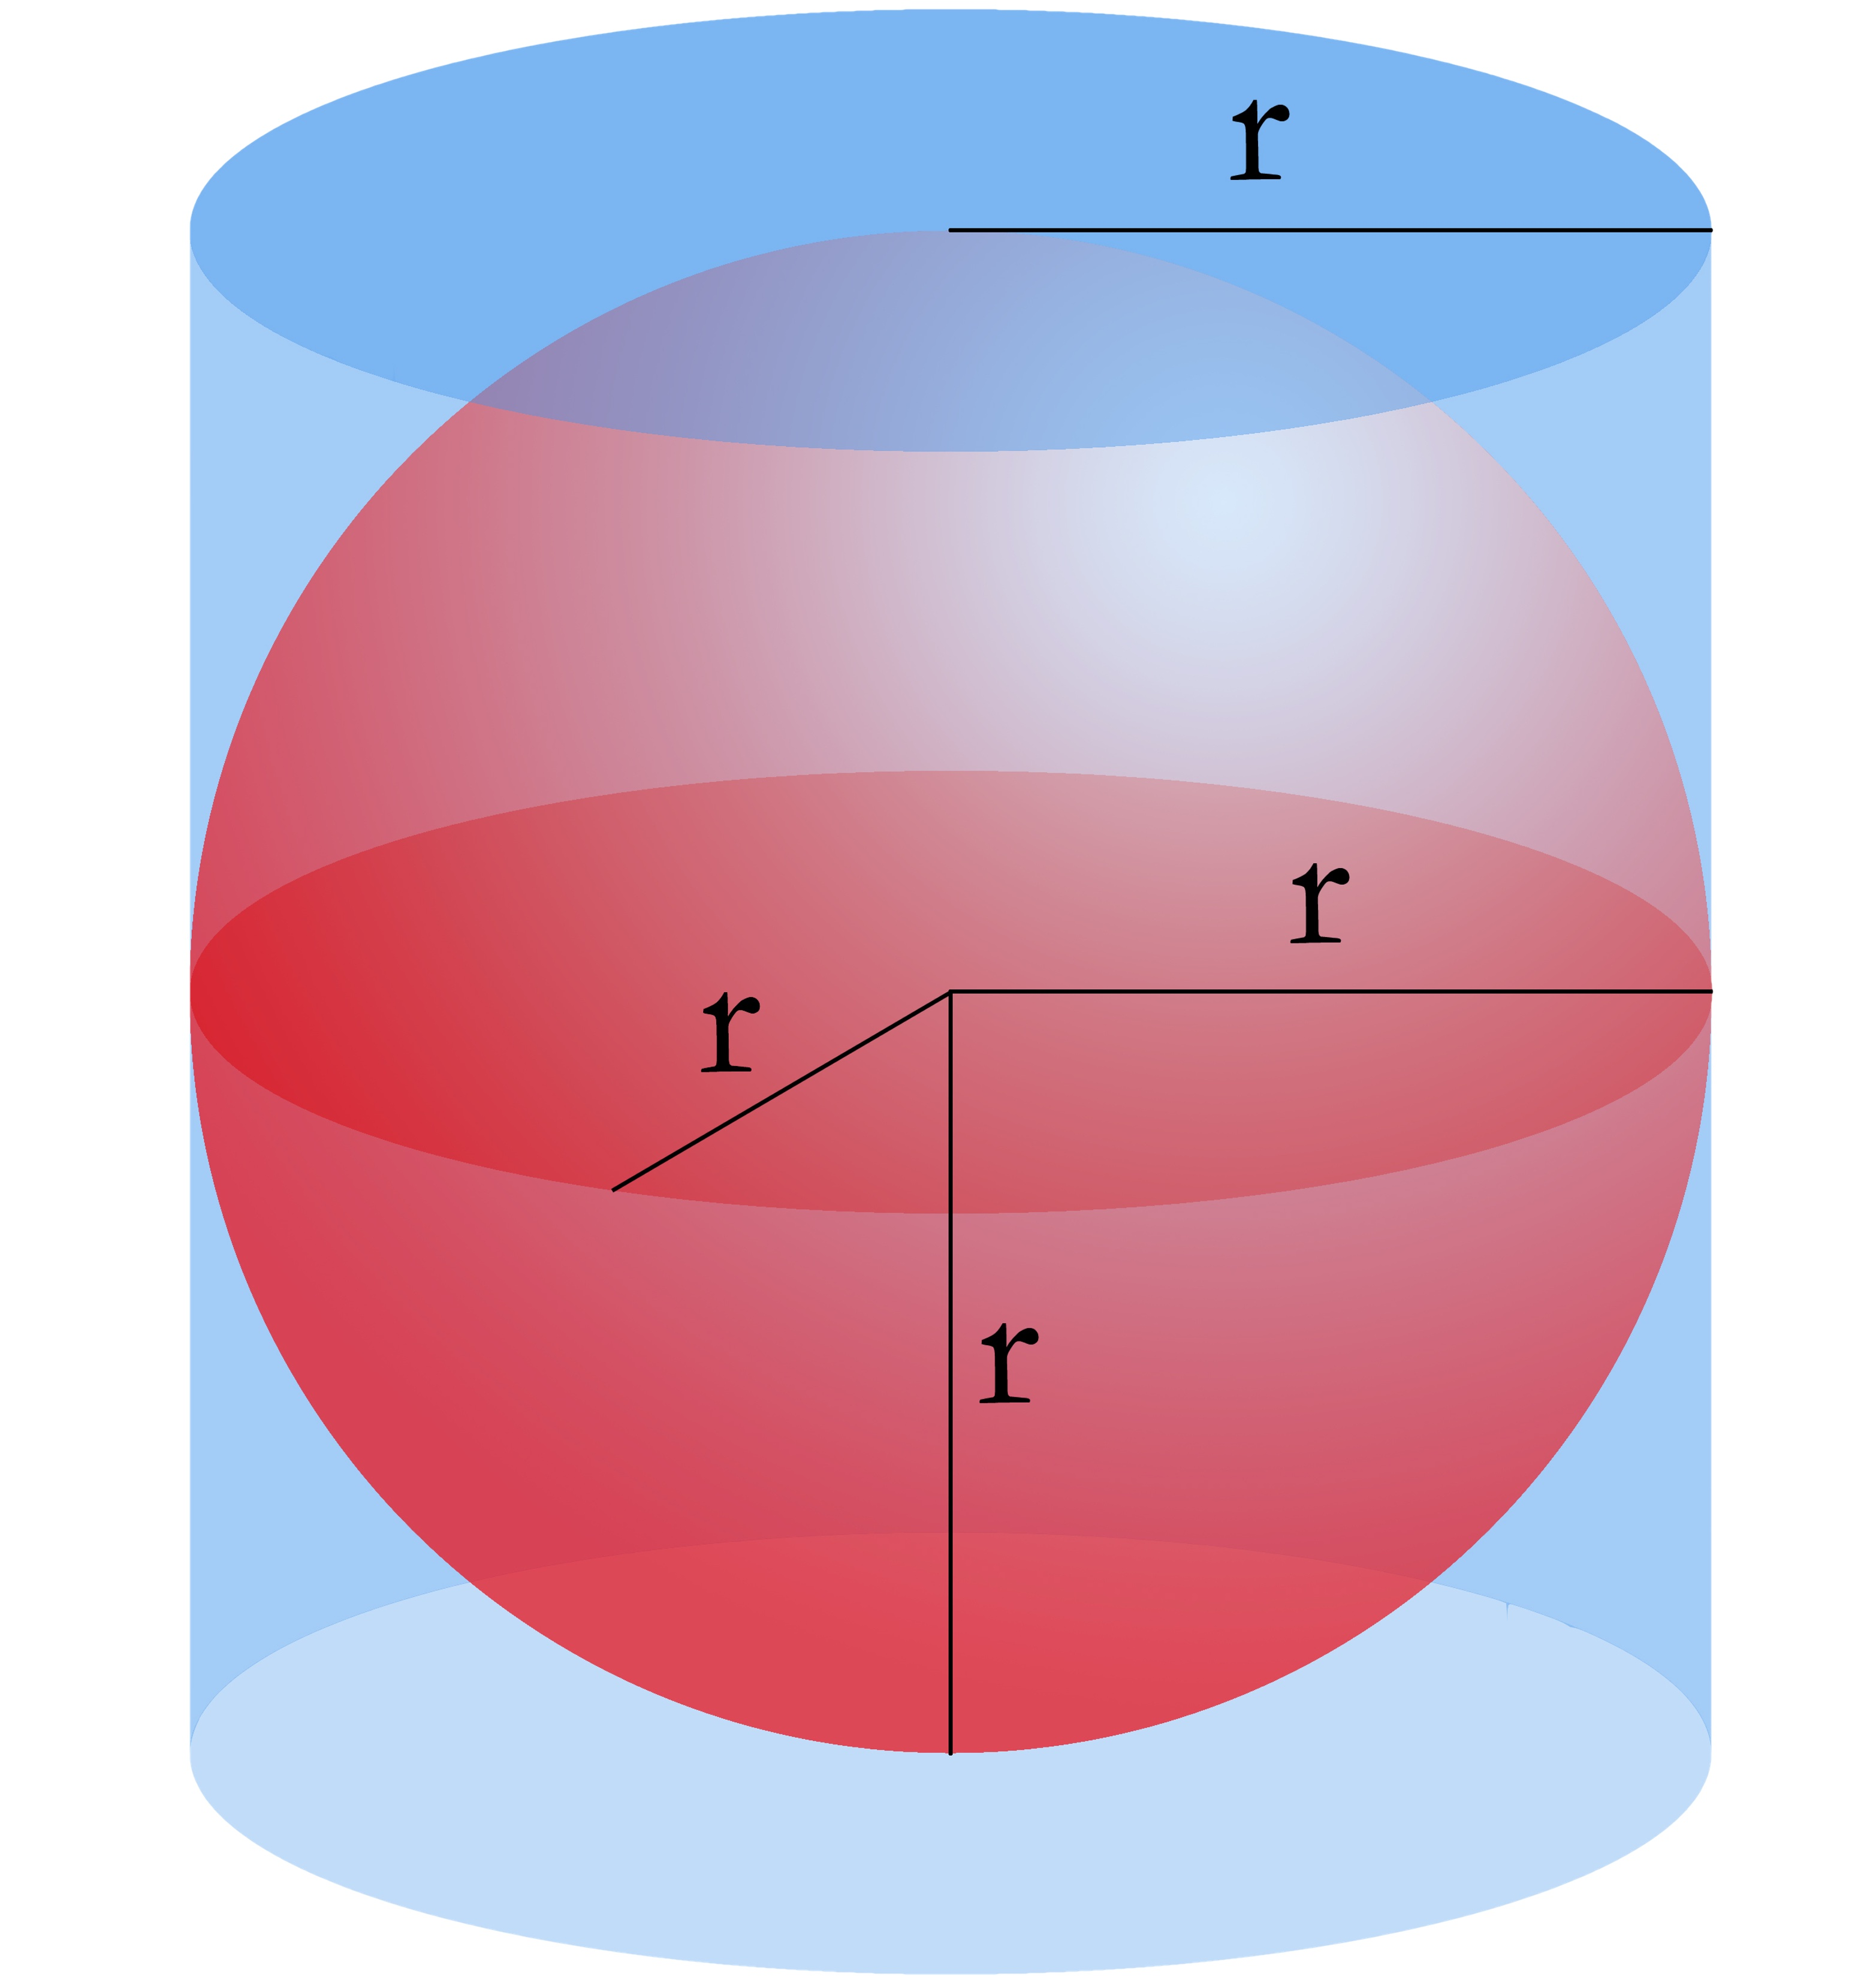
\includegraphics[width=0.3\textwidth]{./graph/archimedes}
  \caption{Archimedes' circumscribed cylinder to a ball, \citep{wiki:archimedes}}
  \label{fig:archimedes}
\end{figure}

\theme{Notation:} a ball is defined by one parameter: its radius; while a cylinder by two: its radius and height. Then, denote the ball radius by $\rball$, its volume by $\vball$, the cylinder radius by $\rcyl$, its height by $\hcyl$, and its volume by $\vcyl$.

\theme{Express constraints mathematically.} By looking at \cref{fig:archimedes}, circumscription translates to math as
%
\begin{equation}\label{eq:volumetricratioconstraint}
  \rball = \rcyl = \radius\quad\text{and}\quad\hcyl = 2\radius.
\end{equation}

% subsection terms_and_notation (end)


\subsection{Guessing} % (fold)
\label{sub:guessing}
%
\theme{Exploit math object properties and problem hypotheses.} Volumes are represented by real numbers. Real numbers can be ordered. Thus, volumes can be ordered as well. 

\theme{Argue via inequalities.} Note that volumes are nonnegative, $\vball,\vcyl\geq 0$, that the ball and the cylinder are nonempty, hence their volumes are nonzero, $\vball,\vcyl > 0$, and that the cylinder contains the ball, thus $\vcyl > \vball$. Therefore, order the volumes as 
%
\begin{equation*}
  \vcyl > \vball > 0\,.
\end{equation*}
%
\theme{Nondimensionalize.} Since $\vcyl > 0$, rearrange the last inequality to
%
\begin{equation}\label{eq:guesstimate}
  0 < \dfrac\vball\vcyl < 1\,.
\end{equation}
%
\theme{Bind variables.} In words, the volumetric ratio lies between 0 and 1. 

\theme{Reflect.} \Cref{eq:guesstimate} does not give the exact value for the volumetric ratio, but it does say where the value should and should not lie.

% section guessing (end)


\subsection{Refining guess} % (fold)
\label{sub:refining_guess}
%
\theme{Squeeze good graphs.} Confirm in \cref{fig:archimedes} that $\vball < \vcyl$. Notice also that $\vball$ is greater than $\vcyl/2$. Therefore, refine the estimate to $\vcyl/2 < \vball < \vcyl$, or
%
\begin{equation}\label{eq:firstestimate}
  \dfrac 12 < \dfrac{\vball}{\vcyl} < 1\,;
\end{equation}
%
\ie, the volumetric ratio lies between 0.5 and 1.

% subsection refining_guess (end)


\subsection{Scaling} % (fold)
\label{sub:scaling}
%
\theme{Use DA and scaling.} Aided by dimensional analysis, find how ball and cylinder volumes scale.

\theme{Constrain and approximate early.} By \cref{eq:volumetricratioconstraint}, the ball volume and the cylinder volume scale with $\radius^3$: $\vball,\vcyl\scale\radius^3$. Their ratio thus scales as
%
\begin{equation*}
  \dfrac{\vball}{\vcyl}\scale\dfrac{\radius^3}{\radius^3}\scale 1\,;
\end{equation*}
%
\theme{Interpret.} \ie, the ratio scales with unity: it is a constant. 

\theme{By DA}, replace the scaling symbol for an equality and a dimensionless quantity $\kdim$:
%
\begin{equation}\label{eq:secondestimate}
  \dfrac{\vball}{\vcyl} = \kdim\,,
\end{equation}
%
which gives a second estimate for the volumetric ratio. 

\theme{Confirm and chain previous work.} \Cref{eq:secondestimate} agrees with the refined guess, \cref{eq:firstestimate}. It therefore suggests a bind: $0.5 < \kdim < 1$.

\theme{Hints on how to scale:} in general, given a circular cylinder, its height and radius have $\dim\height = \dim\radius = \phdim L$; while its volume $\dim\volume = \phdim{L^3}$. Thus, to satisfy dimensional homogeneity, either $\volume\scale\height^2\radius$ or $\volume\scale\height\radius^2$. To resolve ambiguity, note that, since the cylinder is circular, it can be thought of as a set of stacked disks. Finally, because the disk area scales with its squared radius, the cylinder volume scales as $\volume\scale\height\radius^2$.

% subsection scaling (end)


\subsection{Dimensional analysis} % (fold)
\label{sub:dimensional_analysis}
%
\theme{Establish the geometric model.} We look for a geometric model, a function, $f$ among the problem quantities of the form:
%
\begin{equation*}
  f\vat{\vball,\rball,\vcyl,\rcyl,\hcyl} = 0\,.
\end{equation*}

\theme{Find number of $\kdim$s.} Since we are dealing with geometry, a set of dimensionally independent dimensions is $\elset{\phdim L}$ with unity cardinality. We have five problem quantities in our model. Thus, according to Buckingham's Pi theorem, we need ($5 - 1 =$) 4 dimensionless quantities, $\kdim$.

\theme{Construct $\kdim$s.} We propose the following $\kdim$s:
%
\begin{equation*}
  \kdim_1 = \dfrac{\vball}{\vcyl}\,,\quad
  \kdim_2 = \dfrac{\rball}{\rcyl}\,,\quad
  \kdim_3 = \dfrac{\rball}{\hcyl}\,,\quad\text{and}\quad
  \kdim_4 = \dfrac{\rcyl}{\hcyl}\,.
\end{equation*}
%
\theme{Dimensionless geometric model.} Again, by the Pi theorem, we use the $\kdim$s to express the geometric model in an equivalent dimensionless form:
%
\begin{equation*}
  f\vat{\dfrac{\vball}{\vcyl}, \dfrac{\rball}{\rcyl}, \dfrac{\rball}{\hcyl}, \dfrac{\rcyl}{\hcyl}} = 0\,.
\end{equation*}
%
\theme{Constrain the model.} If we now constrain the model, \cref{eq:volumetricratioconstraint}, then the last equation becomes $f\vat{\vball/\vcyl} = 0$, which corresponds to
%
\begin{equation}\label{eq:thirdestimate}
  \dfrac{\vball}{\vcyl} = \kdim\,.
\end{equation}

\theme{Confirm previous work.} \Cref{eq:thirdestimate} agrees with the refined guess, \cref{eq:firstestimate}, and scaling, \cref{eq:secondestimate}.

\theme{Reflect.} Intentionally, we did not \emph{constrain early} the model, thus our calculation was long. Had we done so, we would have had a shorter, cleaner solution.

% subsection dimensional_analysis (end)


\subsection{Differential geometry} % (fold)
\label{sub:differential_geometry}
%
\theme{Admit \scare{defeat}.} We used approximate methods to find that the volumetric ratio is a constant and to estimate the constant value should be. However, the exact number still escapes us.

\theme{Correct.} To find the precise value, we use differential geometry.

In cylindrical coordinates, a circular cylinder $\region C$ of height $\hcyl$ and radius $\rcyl$ can be represented by the set
%
\begin{equation*}
  \region C = \desset{\tuple{\cxpos,\cypos,\czpos}\in\nespace 3}
                     {0\leq\cxpos\leq\rcyl,
                      0\leq\cypos\leq 2\pi,
                      0\leq\czpos\leq\hcyl
                     }\,,
\end{equation*}
%
where the set has been properly oriented.
%
The metric for cylindrical coordinates is $\metric\sbtxt{cyl} = \diag\vat{1,\cxpos,1}$. Therefore, the volume of the cylinder can be calculated from the cylinder volume form as
%
\begin{equation*}
  \vcyl = \int_{\region C}\sqrt{\det\metric\sbtxt{cyl}}\,d\cxpos\oprod d\cypos\oprod d\czpos
        = \int_{0}^{\rcyl}\cxpos\,d\cxpos \int_{0}^{2\pi}d\cypos \int_{0}^{\hcyl}d\czpos 
        = \dfrac 12 \rcyl^2 2\pi \hcyl
        = \pi\rcyl^2\hcyl\,.
\end{equation*}

In spherical coordinates, a ball $\region B$ of radius $\rball$ can be described as
%
\begin{equation*}
  \region B = \desset{\tuple{\sxpos,\sypos,\szpos}\in\nespace 3}
                     {0\leq\sxpos\leq\rball,
                      0\leq\sypos\leq 2\pi,
                      0\leq\szpos\leq \pi
                     }\,,
\end{equation*}
%
where the set has been properly oriented.
%
The metric for spherical coordinates is $\metric\sbtxt{sph} = \diag\vat{1,\sxpos,\sxpos\sin\sypos}$. Therefore, the volume of the cylinder can be calculated from the cylinder volume form as
%
\begin{equation*}
  \vcyl = \int_{\region C}\sqrt{\det\metric\sbtxt{sph}}\,d\sxpos\oprod d\sypos\oprod d\szpos
        = \int_{0}^{\rball}\sxpos^2\,d\sxpos \int_{0}^{2\pi} d\sypos \int_{0}^{\pi}\sin\szpos\,d\szpos 
        = \dfrac 13\rball^3 2\pi 2
        = \dfrac 43\pi\rball^3\,.
\end{equation*}
%
Therefore, after applying the embedding constraint, the volumetric ratio is given by
%
\begin{equation}\label{eq:volsbydifferentialgeometry}
  \dfrac{\vball}{\vcyl} = \dfrac{4\pi}{3\pi}\dfrac{\rball^3}{\rball^2\rball}
                        = \dfrac 23\,.
\end{equation}
%
\theme{Confirm previous work.} \Cref{eq:volsbydifferentialgeometry} agrees with our estimates, \cref{eq:firstestimate,eq:secondestimate}. In fact, it gives us the value for the dimensionless constant of \cref{eq:secondestimate}, $\kdim = 2/3$. 

\theme{Reflect.} However, we found the constant value at the expense of the differential geometry: more concepts, formalism, and calculations than approximate methods.

% subsection differential_geometry (end)


\subsection{Elegant solution} % (fold)
\label{sub:elegant_solution}

\theme{Refine solution.} Rely on tailor made theorems to improve the solution: less verbosity, less calculations.

\theme{Go fully abstract.} The volume of a $n$-dimensional ball of radius $\radius$ in $\nespace n$ is
%
\begin{equation*}
  \volume_{n}\vat{\radius} = \dfrac{\pi^{n/2}}{\Gamma\vat{\dfrac n2 + 1}}\radius^n\,,
\end{equation*}
%
where $\Gamma$ is the gamma function. Then, the volume of a three dimensional ball of radius $\rball$ becomes
%
\begin{equation}\label{eq:volumeballbyvolumeofndimensionalball}
  \vball\vat\rball = \dfrac{\pi^{3/2}}{\Gamma\vat{\dfrac 32 + 1}}\rball^3
                   = \dfrac 43\pi\rball^3\,.
\end{equation}

\theme{Build on past work.} For the \emph{circular} cylinder of height $\hcyl$ and radius $\rcyl$, the parallel section area to the cylinder base is $\pi\rcyl^2$. Thus, by Cavalieri's principle, the cylinder volume is the section area times the cylinder height; \ie,
%
\begin{equation}\label{eq:volumecylindercavalieri}
  \vcyl = \pi\hcyl\rcyl^2\,.
\end{equation}
%
Then, constrain \cref{eq:volumeballbyvolumeofndimensionalball,eq:volumecylindercavalieri} by \cref{eq:volumetricratioconstraint} to have the volumetric ratio:
%
\begin{equation}\label{eq:elegantsolution}
  \dfrac\vcyl\vball = \dfrac 23\dfrac{\radius^3}{\radius\radius^2}
                    = \dfrac 23\,.
\end{equation}

\theme{Confirm previous work.} \Cref{eq:elegantsolution} accords with the differential geometry solution, \cref{eq:volsbydifferentialgeometry}.

\theme{Reflect.}

% subsection elegant_solution (end)


Axiomatic definition of volumes: \cite[p. 112]{apostol:1967}.


% section archimedes_s_principle (end)

